\section{Architecture}
\label{sec:arch}
Globally, the architecture of the project follows the MVC (Model-View-Controller) \cite{mvc} paradigm. Its fine granularity favorite the Single-Reponsibility Principle . The project is divided in four packages:

\begin{figure}[H]
\dirtree {%
.1 ..
.1 core.
.1 hunt.
.1 particles.
.1 wator.
}
\end{figure}
\begin{description}

	\item[$core$] contains the logic which is common between the three applications
	\item[$hunt$] contains the logic related to the hunt application
	\item[$particles$] contains the logic related to the particles application
	\item[$wator$] contains the logic related to the wator application
\end{description}

\subsection{Core}

   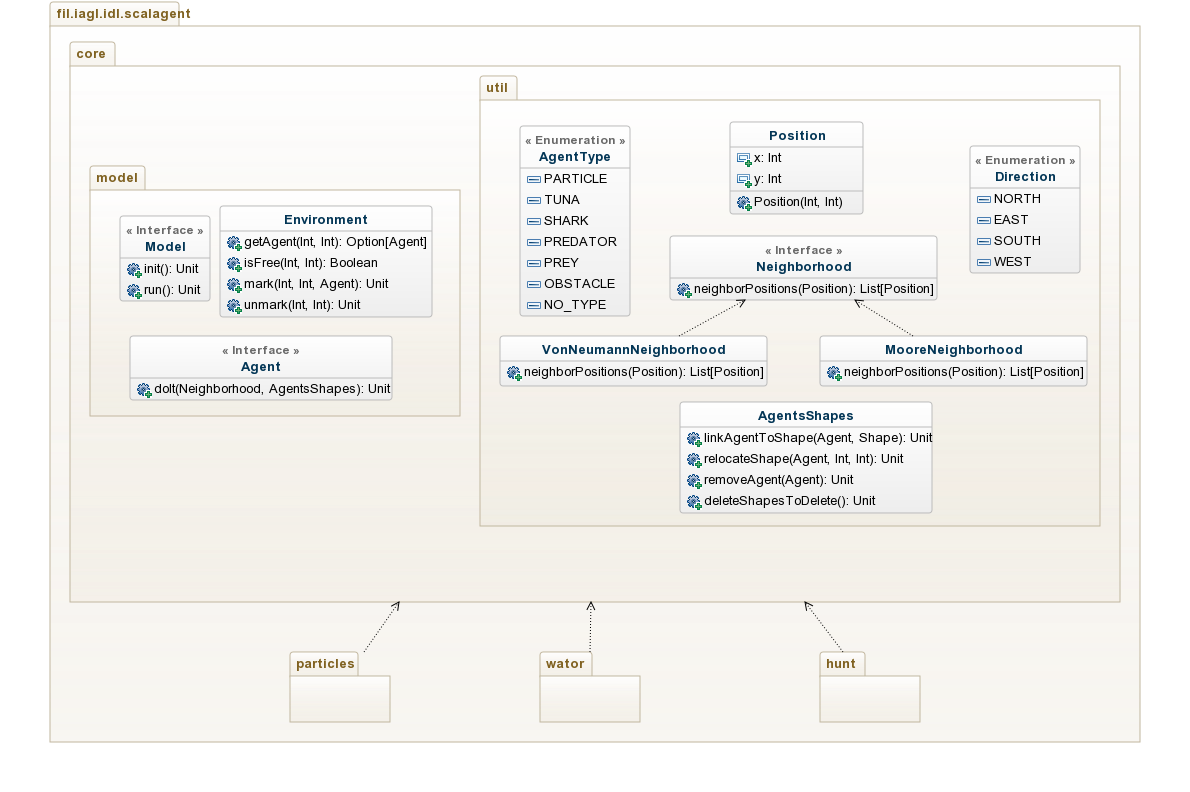
\includegraphics[width=\linewidth]{overview.png}

\begin{figure}[H]
\dirtree {%
.1 ..
.1 model.
	.2 Agent.scala : an agent in a multi-agent system.
	.2 Environment.scala : an environment in the multi-agent system.
	.2 Model.scala : the model of the application within the MVC paradigm.
.1 util.
    .2 AgentsShapes.scala : the shapes representing the agents.
    .2 AgentType.scala : the type of an agent.
    .2 Direction.scala : the direction of an agent.
    .2 MooreNeighborhood.scala : the Moore neighborhood of an agent.
    .2 Neighborhood.scala : the neighborhood of an agent.
    .2 Observable.scala : the observable within the Observer pattern.
    .2 Observer.scala : an observer neighborhood within the Observer pattern.
    .2 Position.scala : the position of an agent.
    .2 VonNeumannNeighborhood.scala : the Von Neumann neighborhood of an agent.
}
\end{figure}

\newpage

\subsection{Particles}

   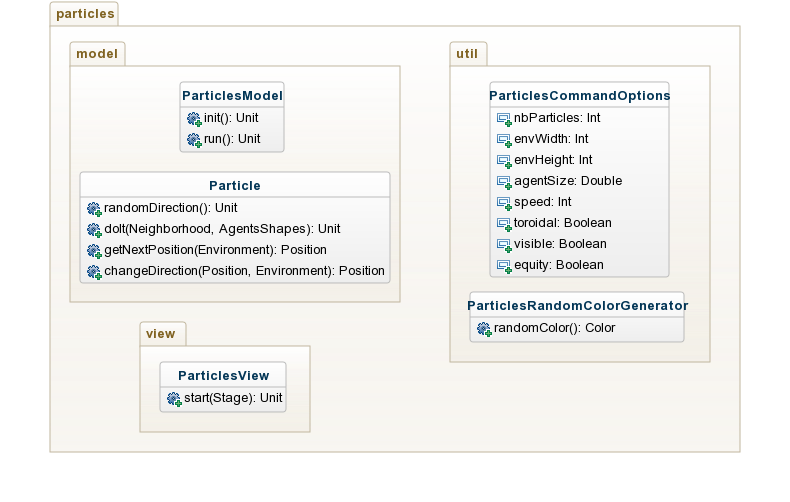
\includegraphics[width=\linewidth]{particles_diagram.png}

\begin{figure}[H]
\dirtree {%
.1 ..
.1 model.
	.2 Particle.scala : a particle.
	.2 ParticlesModel.scala : the model of the particles application within the MVC paradigm.
.1 util.
	.2 ParticlesCommandOptions.scala : the options that can be applied to the particles application.
	.2 ParticlesRandomColorGenerator.scala : a random color generator for particles.
.1 view.
    .2 ParticlesView.scala : the view of the wator application within the MVC paradigm.
}
\end{figure}
\newpage

\subsection{Wator}
   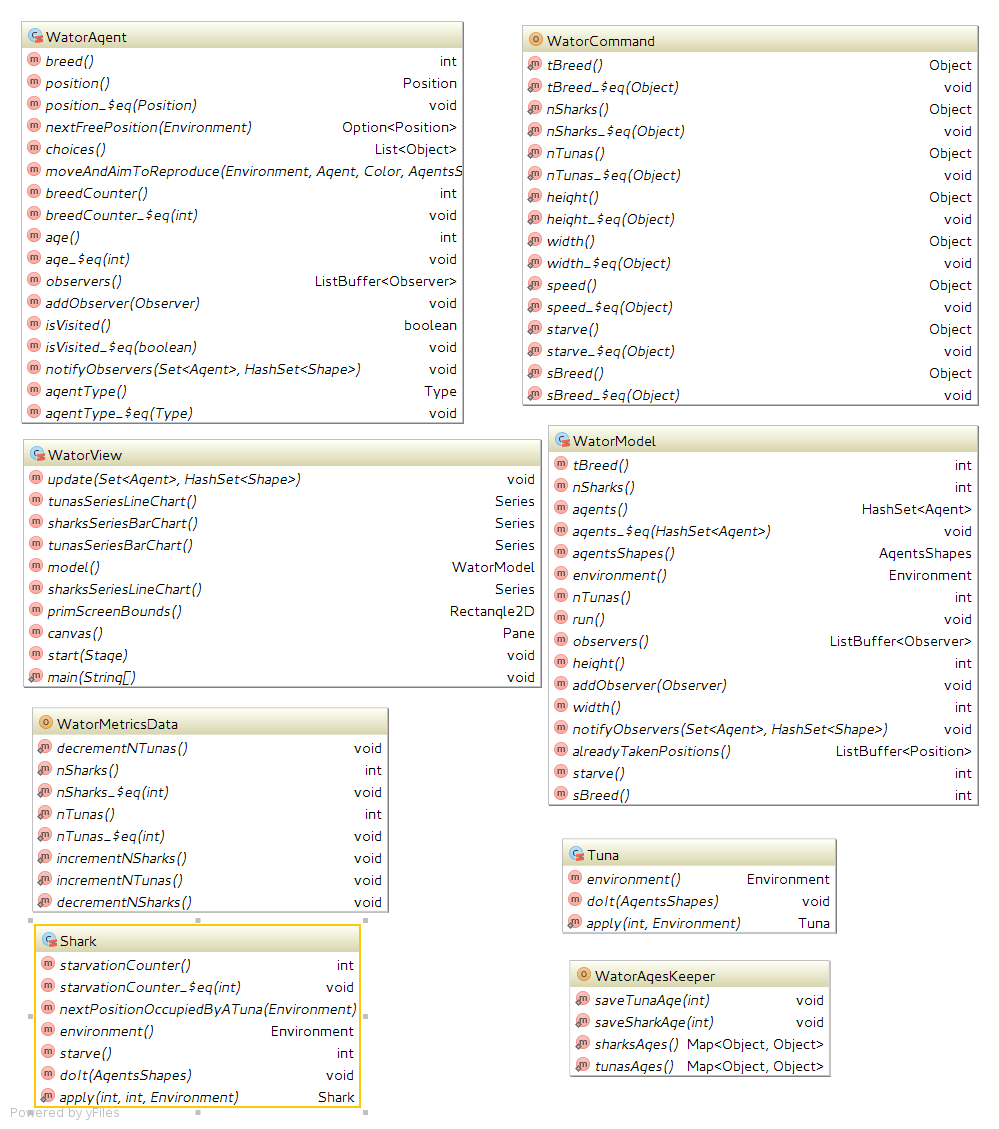
\includegraphics[width=\linewidth]{wator_diagram.png}

\begin{figure}[H]
\dirtree{%
.1 model.
	.2 Shark.scala : a shark.
	.2 Tuna.scala : a tuna.
	.2 WatorAgent.scala : a agent in the wator environment (an agent that can reproduce).
	.2 WatorModel.scala : the model of the wator application within the MVC paradigm.
.1 util.
	.2 WatorAgesKeeper.scala : data for the age pyramid.
	.2 WatorCommandOptions.scala : the options that can be applied to the wator application.
	.2 WatorMetricsData.scala : data for the time-dependent number of tunas and sharks.
.1 view.
    .2 WatorView.scala : the view of the wator application within the MVC paradigm.
}
\end{figure}
\newpage

\subsection{Hunt}

   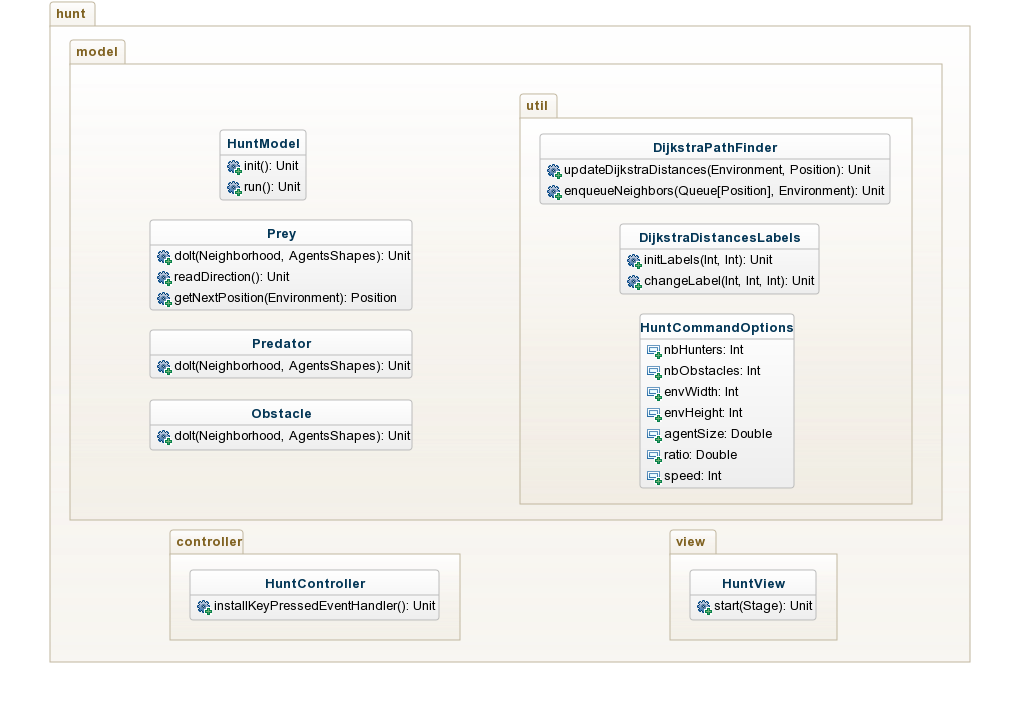
\includegraphics[width=\linewidth]{hunt_diagram.png}

\begin{figure}[H]
\dirtree{%
.1 ..
.1 controller.
	.2 HuntController.scala : the controller of the hunt application within the MVC paradigm.
.1 model.
	.2 HuntModel.scala : the model of the hunt application within the MVC paradigm.
	.2 Obstacle.scala : an obstacle.
	.2 Predator.scala : a predator.
	.2 Prey.scala : a prey.
.1 util.
	.2 DijkstraDistancesLabels.scala : the Dijkstra distances labels drawing.
	.2 DijkstraPathFinder.scala : the Dijkstra path finder.
	.2 HuntCommandOptions.scala : the options that can be applied to the hunt application.
.1 view.
	.2 HuntView.scala : the view of the hunt application within the MVC paradigm.
}
\end{figure}

\newpage